\chapter{Capsule Network Architectures}\label{chapter:capsules}
A capsule is conceived as a group of neurons whose outputs encode different properties of an entity such as an object or part of an object in an image. The properties could represent instantiation parameters on the object's appearance manifold like the precise pose, lighting and deformation or the probability that the entity is present. Layers within a capsule network consist of several capsules. Routing between the layers is determined by the votes from the capsules in the lower layer. Capsules can make a guess as to what they expect the higher layer's capsules instantiation parameters to be and cast a vote. Votes are calculated by applying discriminatively learned transformations to a capsule's neuron's outputs. The routing algorithm will then determine, based on the lower capsules' votes, which higher layer capsules to activate. The goal of capsules is to achieve invariance in the presence probability of the object they represent regarding the object's instantiation parameters. A specific capsule architecture is largely defined by the nature of its routing algorithm and the dimension of its output as well as the order of the tensors used to compute the votes.

\section{Transforming Auto-encoders}
The first publication on capsules came from Hinton et al. in the form of transforming auto-encoders in 2011 \cite{hinton2011transforming}. These capsules encode the instantiation parameters of their internal representation together with the probability that the learned entity is present into a small output vector. Each capsule would learn to recognize a single visual entity over a limited subdomain of its appearance manifold. Ideally, the probability would be locally invariant as long as the instantiation parameters remain within the trained submanifold. This is in contrast to the instantiation parameters, which are equivariant. Meaning as the viewing conditions change, the parameters encoding the appearance change by an equal amount.

The transforming auto-encoders introduced by Hinton et al. in 2011 were already motivated by a desire to retain precise part-whole relationships, which are lost by the pooling operations in convolutional neural networks (cf. section \ref{section:limitations}). If a capsule can be trained to encode the pose of the visual entity it represents in its output vector, it is a simple matter to test whether two capsules $A$ and $B$ are in agreement about a higher level capsule $C$. To see this, suppose that the matrix $\vb{T}_{A/B}$ is the pose between the canonical entity as learned by the capsule $A$ or $B$ respectively and the current instantiation. Multiplying this with the part-whole transformation matrix $\vb{T}_{A/B\rightarrow C}$ will result in a prediction for the pose of capsule $C$'s entity. Now, if
\begin{align}
    \vb{T}_A\vb{T}_{A\rightarrow C} \approx \vb{T}_B\vb{T}_{B\rightarrow C},
\end{align}
then the capsules are a close match and activate capsule $C$. Hinton et al. argue that this naturally leads to precise part-whole relationships. If the entities of capsules $A$ and $B$ e.g. correspond to a mouth and a nose respectively, then they have to be in right spatial relationship to form a face if they activate the higher capsule $C$ representing the whole face. The pose of capsule $C$ can then be determined by the average of the lower capsules' votes.
\begin{align}
    \vb{T_C} = \sum_{i\in \{A, B\}} \vb{T}_i\vb{T}_{i\rightarrow C}
\end{align}
This means that except for the first layer of capsules, only the viewpoint invariant part-whole transformations have to be learned, while the entity poses are encoded in the neural activities at run time. The rest of the paper focuses on how to extract the poses from the pixel intensities for the first layer. This is done by training capsules on transformed image pairs and providing the capsules with non-visual access to the transformation. Hinton et al. justified this by pointing out that the human visual system is also provided with information about the eye-movement while saccades correspond to a translational transformation of the retinal image.
\begin{figure}
    \centering
    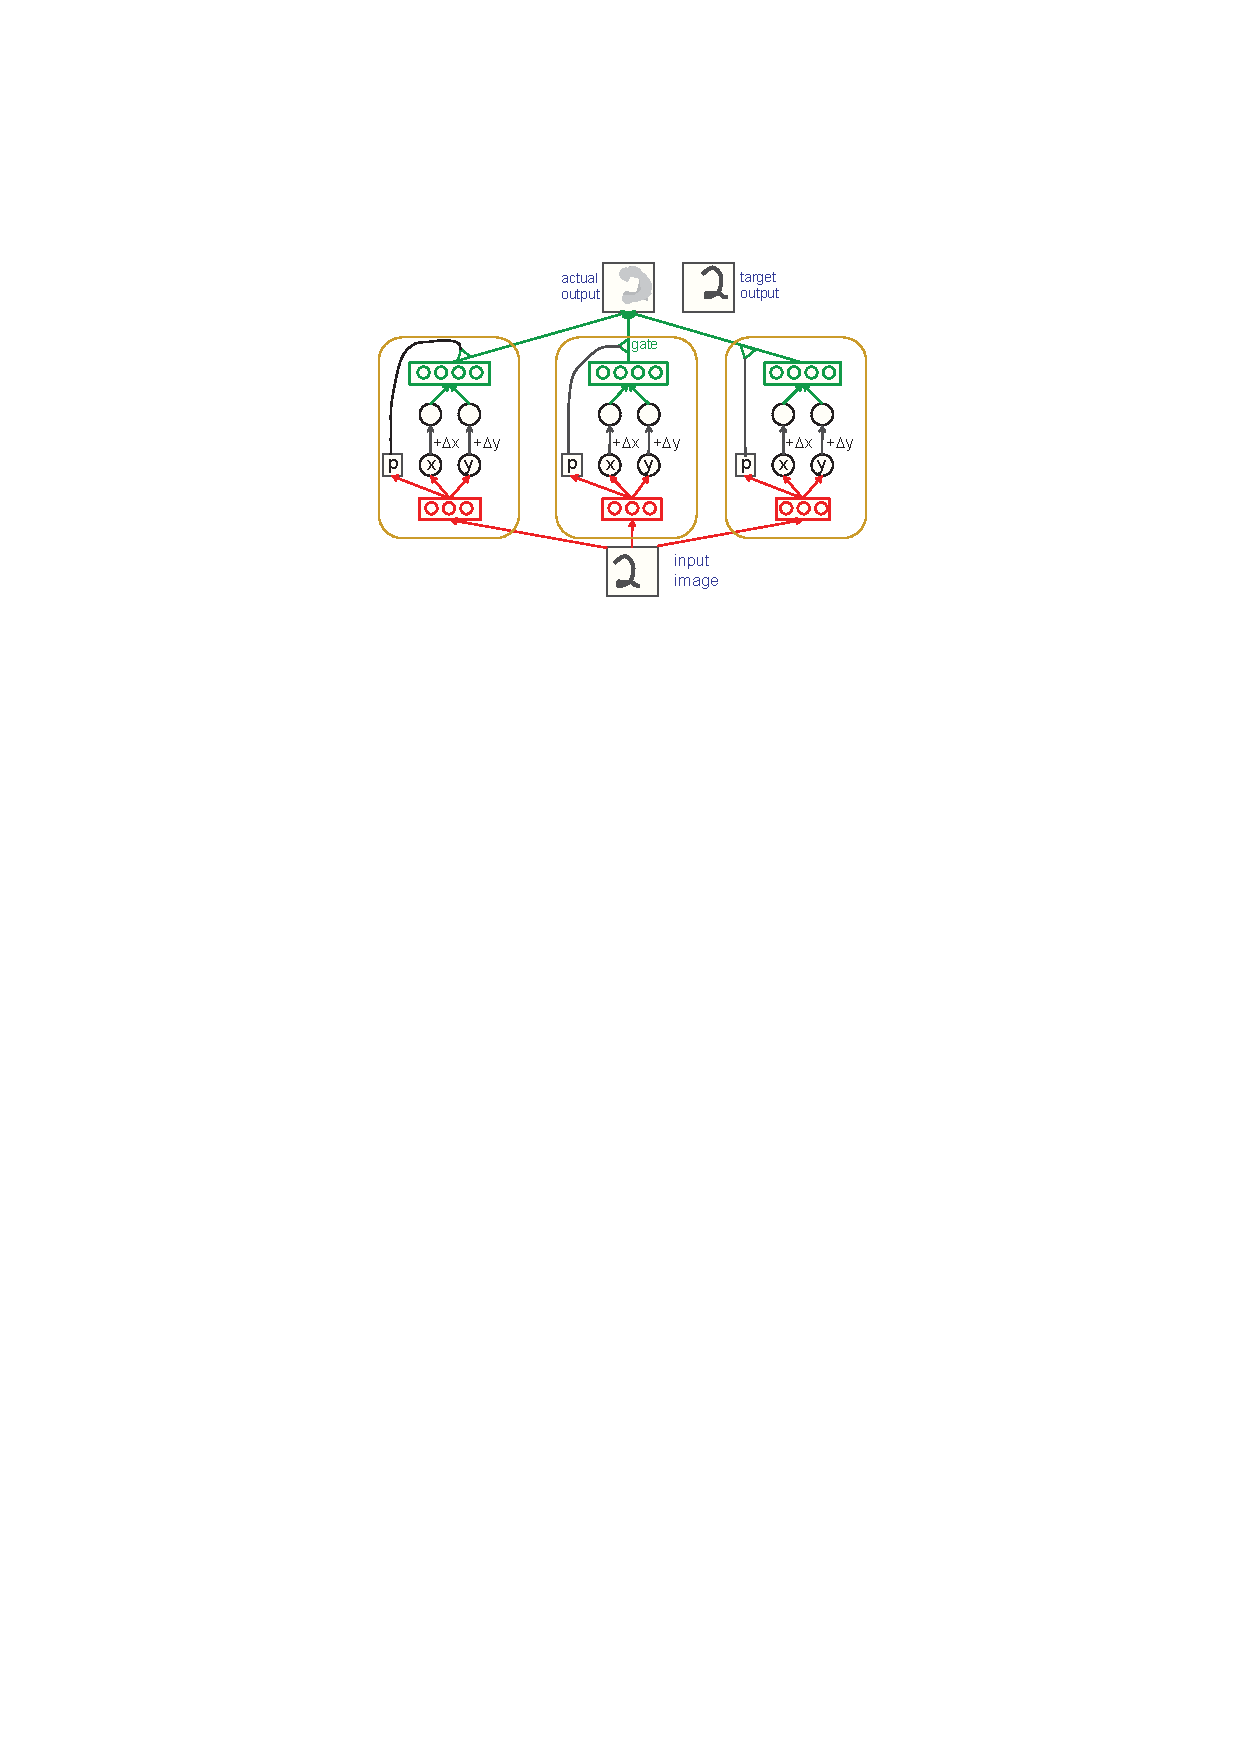
\includegraphics[width=.75\textwidth]{figures/caps-fig1.pdf}
\caption[Capsules in a transforming auto-encoders]{Capsules in a transforming auto-encoder \cite{hinton2011transforming}. The network consists of a single layer of capsules. Each capsule includes hidden recognition (in red) and generation units (in green). During training transformation parameters (in this case the translations $\Delta x$ and $\Delta y$) as well as the transformed image are provided to the network. A capsule's output vector is further multiplied with its probability, thus muting capsules with a low probability.}\label{fig:auto-encoders}
\end{figure}\noindent

These first capsule networks actually consist of only one layer of capsules and do not include the routing mechanism of later implementations. Instead, they include two internal layers of logistic neurons, termed recognition and generation units respectively (cf. figure \ref{fig:auto-encoders}). The recognition units are trained to extract pose parameters and the probability that the visual entity is present directly from the provided image. A capsule's input can be constrained to a fixed receptive field with the capsules aligned in a grid across the image. The capsules then apply a transformation to the pose and provide the generation units with this information. The generation units on the other hand are trained to output the transformed part of the input image centered at the capsule's receptive field. All the neurons within a capsule are trained discriminatively using gradient descent with backpropagation. The training signal is provided by a form of reconstruction loss where the capsules have access to the transformation and the input and reconstruction target are the original and transformed images respectively. Transforming auto-encoders are able to learn poses in the form of $3x3$ matrices and can be used to successfully apply affine transformations to input images once trained. However, they are limited to one layer of capsules and cannot be scaled effectively, as the capsules are fixed to a single position, compared to the shared weights of moving filters in convolutional layers. Also they are only able to learn properties, that can be controlled and provided in explicit non-visual form to the network.
\section{Dynamic Routing Between Capsules}
In 2017 Sabour et al. extended upon the transforming auto-encoders by suggesting a dynamic routing algorithm for capsules \cite{sabour2017dynamic}. While the benefit of dynamic routing between capsule layers in regard to part-whole relationships was already elaborated upon by Hinton et al., Sabour et al. also motivated the mechanism biologically. They pointed out that human vision ignores irrelevant details by focusing attention on salient features in a sequence of fixations and only ever processes a fraction of the optic array at the highest resolution. They assumed that with a single fixation, groups of activated neurons build a tree structure within the fixed multi-layer visual system. The paper suggests to implement the nodes of this image parse tree as active capsules and have each capsule choose their parent node based on the routing algorithm. As with the capsules of transforming auto encoders, the capsule's neurons should learn to represent various instantiation parameters such as pose, deformation, velocity, albedo, hue, texture, etc. However, the probability of the instance's presence is encoded in the length of a vector of instantiation parameters. A nonlinearity is applied to the output vector in order to keep the length from exceeding $\num{1}$, while keeping the orientation unchanged.
\begin{align}
    \vb{u}_j = \frac{\norm{\vb{s}_j}^2}{1+\norm{\vb{s}_j}^2}\frac{\vb{s}_j}{\norm{\vb{s}_j}}
    \label{eq:squash}
\end{align}
With $\vb{u}_j$ the output vector of capsule $j$ and $\vb{s}_j$ the sum of its inputs. This \emph{squashing} function will reduce short vectors to almost length zero and squash long vectors to a length slightly below 1. For every capsule $j$ that is not a first layer capsule, the input $\vb{s}_j$ is computed from the votes of the lower level capsules.
\begin{align}
    \vb{s}_j = \sum_i c_{ij} \vb{\hat{u}}_{j|i}
\end{align}
Where $\vb{\hat{u}}_{j|i}$ is the lower capsule $i$'s guess for the higher capsule $j$'s instantiation vector. Votes are calculated by applying a transformation matrix $\vb{W}_{ij}$ on a capsule's output vector, as was suggested by Hinton et al. for transforming auto-encoders.
\begin{align}
    \vb{\hat{u}}_{j|i} = \vb{W}_{ij}\vb{u}_i
\end{align}
In this scheme, so far only the part-whole transformation matrices $\vb{W}_{ij}$ have to be learned. The coupling coefficients $c_{ij}$ for a lower capsule $i$ sum to 1. They describe the influence a vote from capsule $i$ has over capsule $j$ and are iteratively fine-tuned by the routing algorithm during the network's forward pass. For the first iteration, the coupling coefficients are computed as a softmax function over the log prior coupling logits $b_{ij}$.
\begin{align}
    c_{ij} = \frac{\exp(b_{ij})}{\sum_k \exp(b_{ik})}
    \label{eq:coupling-coeff}
\end{align}
The $b_{ij}$ can be trained discriminatively along with the other parameters. But it was found that the priors have little influence over the routing algorithm.

Using a vector as capsule output allows the use of a powerful dynamic routing-by-agreement algorithm. The agreement between capsule $i$ and each possible parent $j$ is calculated using the scalar product of the lower capsule's vote and the higher capsule's current output.
\begin{align}
    a_{ij} = \vb{u}_j^T \vb{\hat{u}}_{j|i}
\end{align}
If the scalar product is large, it induces top-down feedback, increasing the coupling coefficient between the two capsules by adding the agreement to the coupling logit $b_{ij}$ (cf. algorithm \ref{alg:routing-by-agreement}). As the lower capsule's coupling coefficients are computed as a softmax of the logits, this will simultaneously decrease all the other couplings.
\begin{algorithm}
\caption{Dynamic routing-by-agreement}\label{alg:routing-by-agreement}
\begin{algorithmic}[1]
\Procedure{Routing}{$\vb{\hat{u}}_{j|i},r,l$}
\For{capsule $i$ in layer $l$ and capsule $j$ in layer $l+1$}
  \State{$b_{ij}\gets 0$}
\EndFor
\For{$r$ iterations}
  \For{capsule $i$ in layer l}
    \State{$\vb{c}_i \gets \operatorname{softmax}\qty(\vb{b}_i)$}
    \Comment{computes equation \ref{eq:coupling-coeff}}
  \EndFor
  \For{capsule $j$ in layer l+1}
    \State{$\vb{s}_j \gets \sum_i c_{ij} \vb{\hat{u}}_{j|i}$}
  \EndFor
  \For{capsule $j$ in layer l+1}
    \State{$\vb{u}_j \gets \operatorname{squash}\qty(\vb{s}_j)$}
    \Comment{computes equation \ref{eq:squash}}
  \EndFor
  \For{capsule $i$ in layer $l$ and capsule $j$ in layer $l+1$}
    \State{$b_{ij} \gets b_{ij} + \vb{u}_j^T \vb{\hat{u}}_{j|i}$}
  \EndFor
\EndFor
\Return{$\vb{u}_j$}
\EndProcedure
\end{algorithmic}
\end{algorithm}
\begin{figure}
    \centering
    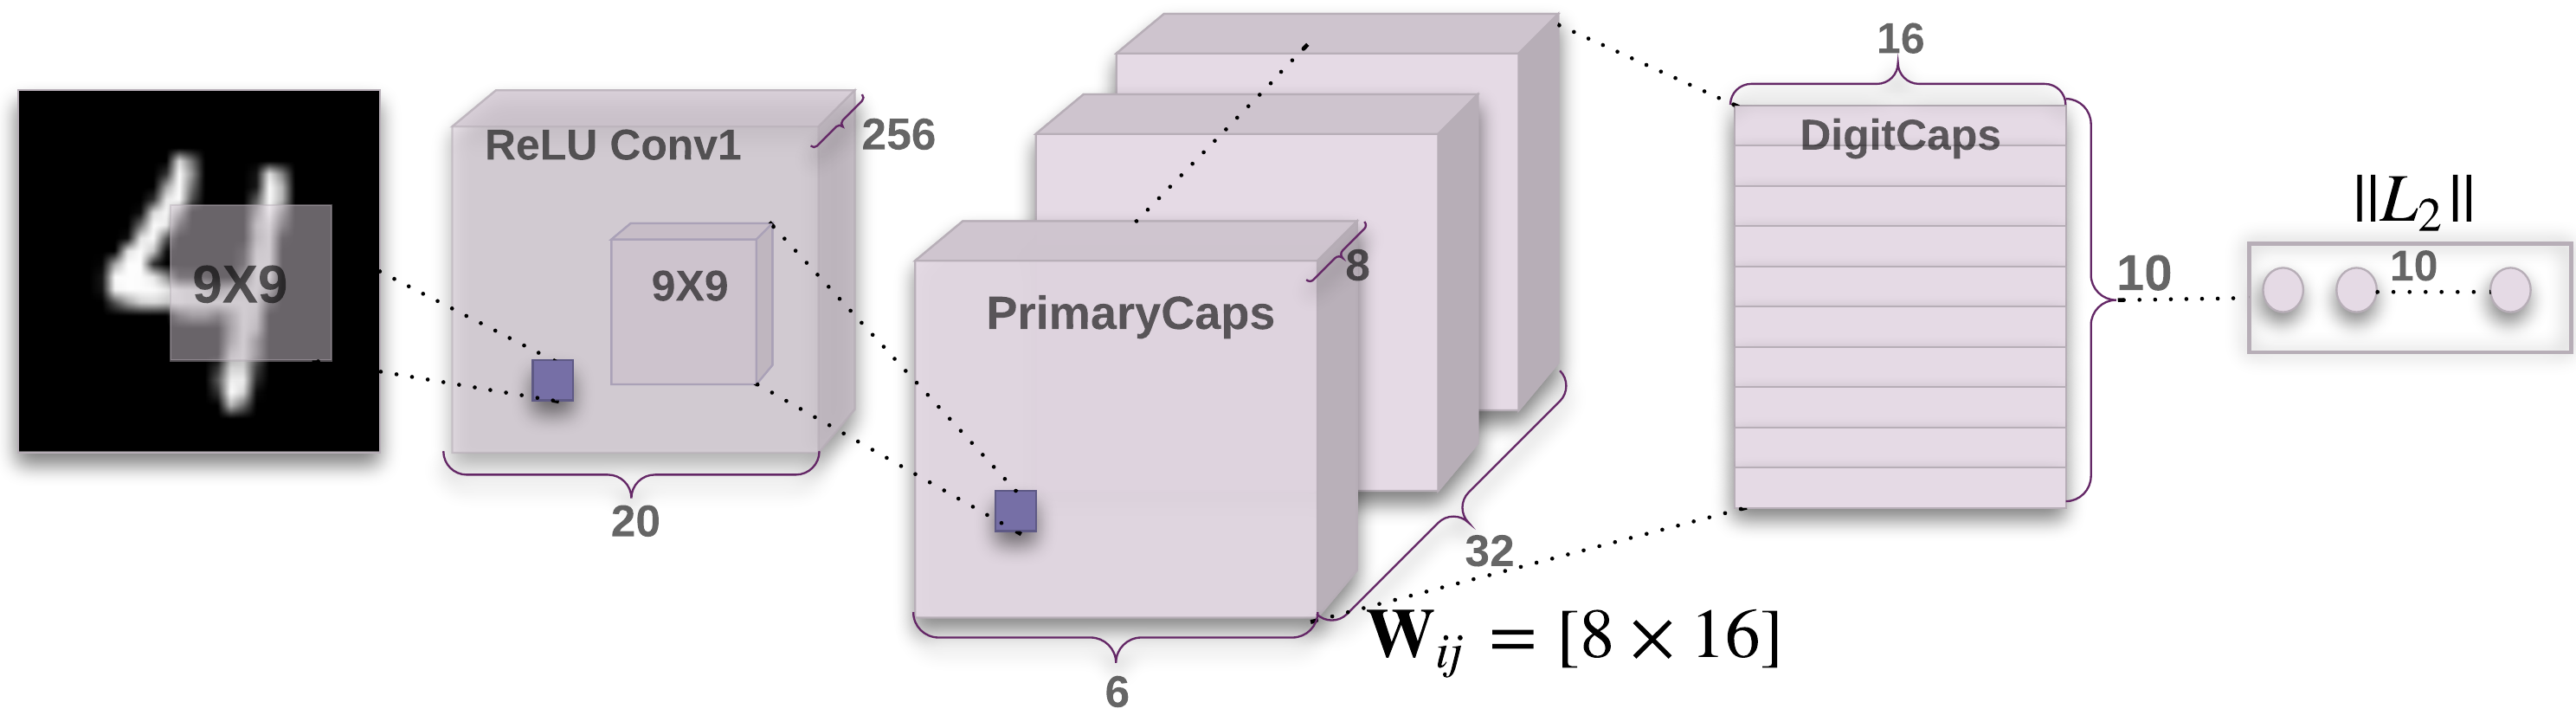
\includegraphics[width=\textwidth]{figures/vector-capsules.png}
\caption[Vector capsule network with 3 layers]{Vector capsule network with 3 layers \cite{sabour2017dynamic}. Conv1 is a standard convolutional layer consisting of $\num{256}$ $9x9$ kernels that learn basic features from pixel intensities, that are converted to $8D$ vector representations by the primary capsule layer. The primary capsule layer is the only convolutional capsule layer in the network and has 32 types of capsules of which each has a receptive field of the size $9x9$ and a stride of $\num{2}$. The class capsule layer (here referred to as DigitCaps) uses $16D$ vectors and $\num{10}$ fully connected capsules. Note that the routing algorithm is applied only between the primary and the class capsule layer.}\label{fig:vector-capsules}
\end{figure}\noindent

Sabour et al. further improved upon transforming auto-encoders by developing convolutional capsule layers. This allows them to use learned features all across the image without losing whole-part relationships. They achieve this by having each capsule of a convolutional layer put out a local grid of vectors to each type of capsule \footnote{The use of different types of capsules within a convolutional layer is analogous to the use of different kernels or filters in CNNs (cf. section \ref{section:cnn}). The resulting map of capsule activities i.e. the lengths of the output vectors can be thought of as a feature map.} in the higher level, where every position on the grid and type of layer is assigned a different part-whole transformation matrix. While this is not strictly convolution, the net effect is the same. Capsules in a convolutional layer possess a receptive field that gets wider the higher up the layer is in the network's topology. For low level capsules, positional information is encoded in the capsule's position within the feature map. The higher up a convolutional capsule is, the smaller the feature map becomes and information on position gets encoded more and more in the instantiation parameter vector.

The primary capsules i.e. the first capsule layer computes its input vectors from the reshaped output of a standard convolutional layer. For the next capsule layers, the routing algorithm is applied. This is yet another improvement over transforming auto-encoders, as the network can be trained on images only without needing access to the applied transformations. The final capsule layer is fully connected and includes one capsule per class (cf. figure \ref{fig:vector-capsules}). \emph{Margin loss} is used to compute the error signal based on the class capsules' output vector length.
\begin{align}
    L_k = T_k \operatorname{max}\qty(0,m^+ - \norm{\vb{v}_k})^2 + \lambda \qty(1-T_k) \operatorname{max}\qty(0, \norm{\vb{v}_k}-m^-)^2
\end{align}
Where $\vb{T} = (0,...,1,...0)^T$ is a one-hot encoded vector of the true class labels and $\lambda$ is used to down-weight the loss for absent classes so that the vectors don't become too short during initial training. In addition Sabour et al. used a reconstruction loss not unlike with transforming auto-encoders in order to encourage the class capsules to encode useful instantiation parameters for each class. This is done by masking out all but the correct class capsule during training and feeding its output vector to a 3-layer decoder (cf figure...). The reconstruction loss is calculated as the euclidean distance between the decoder's output and the input image.

As the internal representation, the votes and the agreement are all vectors, this type of architecture will be referred to as \emph{vector capsules} for the remainder of this thesis.
\begin{figure}
    \centering
    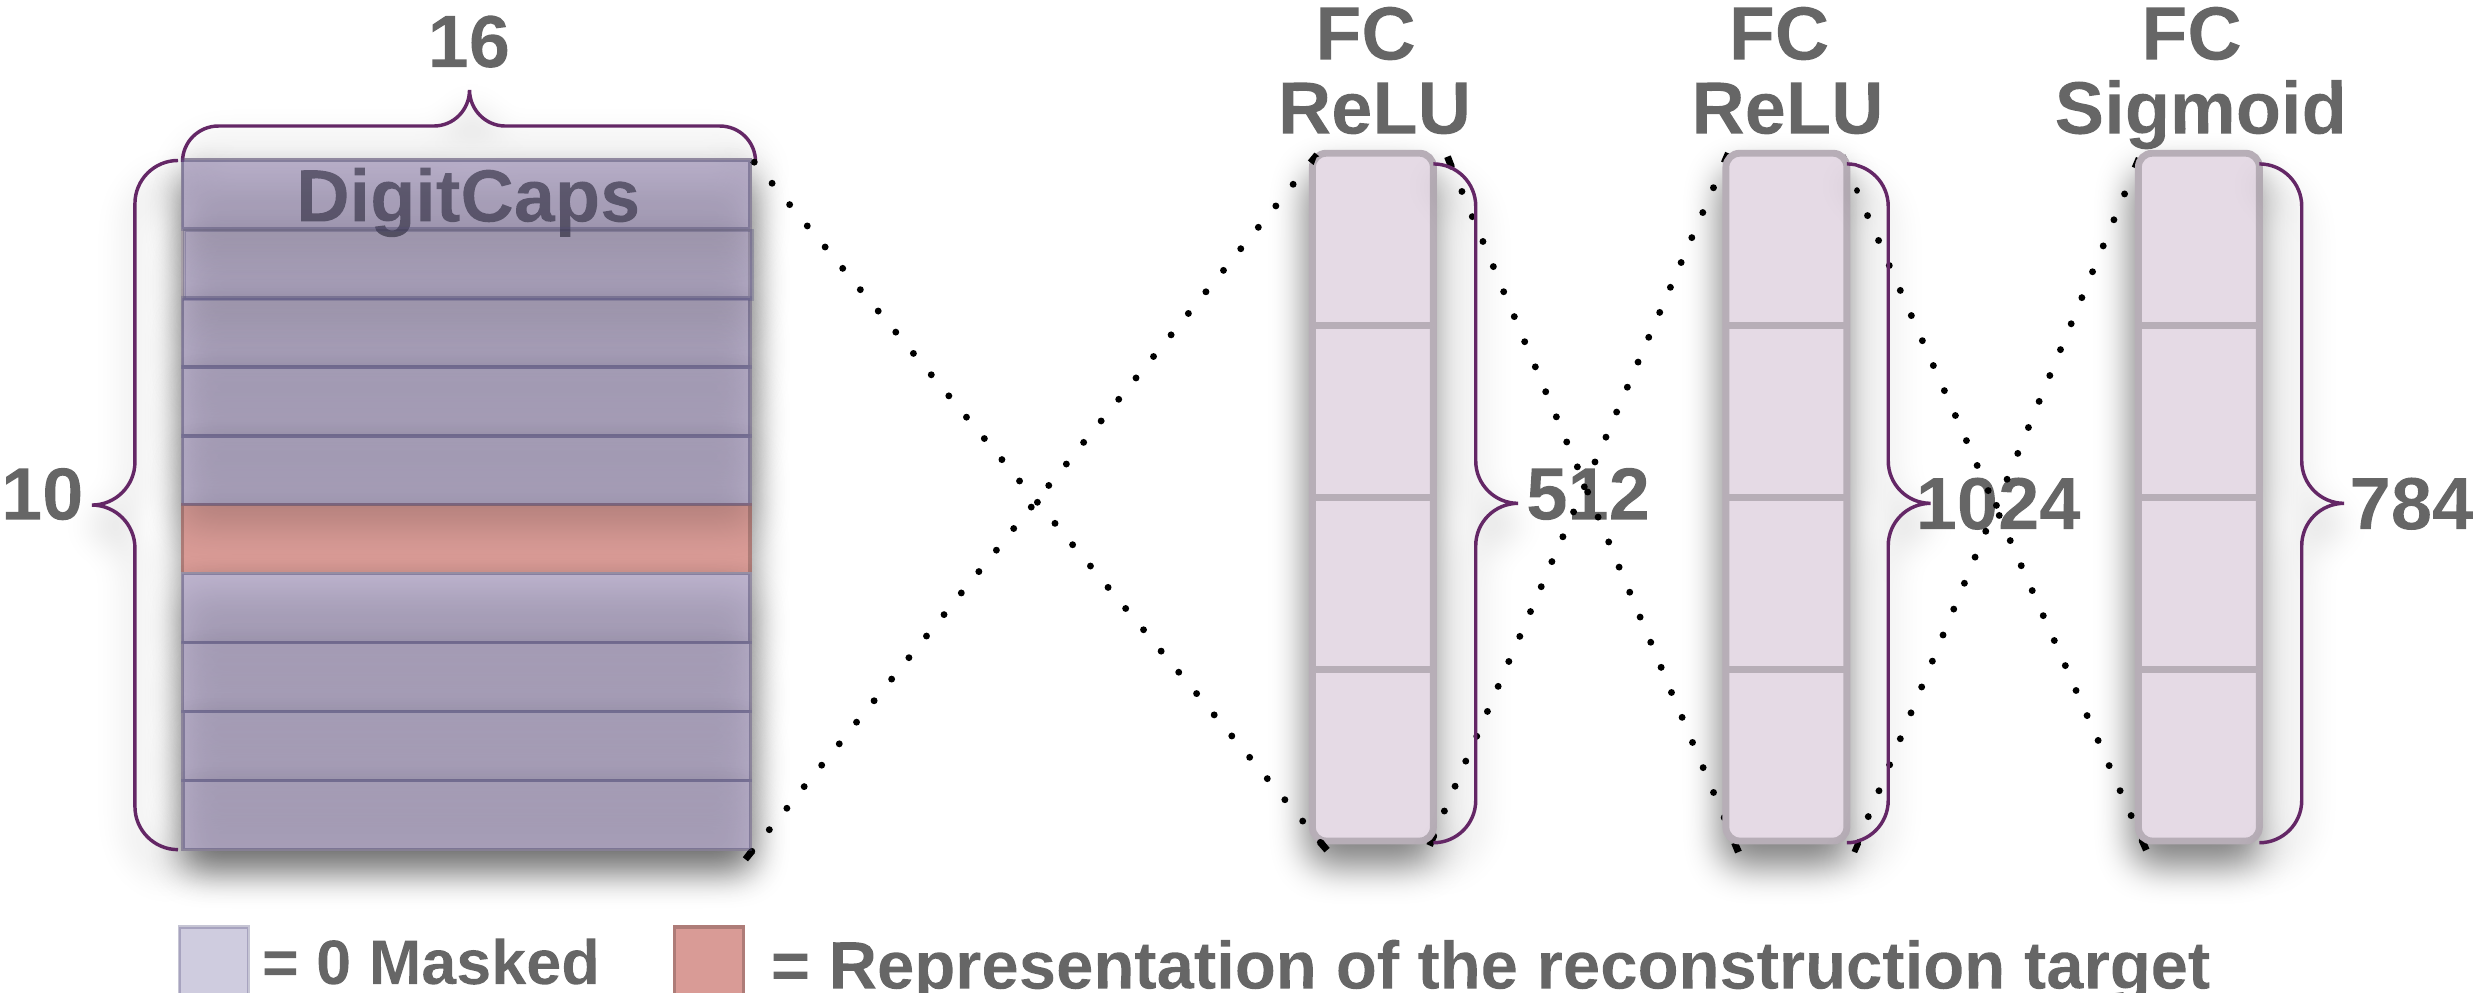
\includegraphics[width=\textwidth]{figures/vector-capsules-reconstr.png}
\caption[Decoder on a class vector capsule layer]{Decoder on a class vector capsule layer \cite{sabour2017dynamic}.}\label{fig:vector-capsules-reconstr}
\end{figure}\noindent
\section{Matrix Capsules With EM Routing}